\documentclass[10pt,a4paper,oneside,fleqn]{article}
\usepackage{geometry}
\geometry{a4paper,left=20mm,right=20mm,top=1cm,bottom=2cm}
\usepackage[utf8]{inputenc}
%\usepackage{ngerman}
\usepackage{amsmath}                % brauche ich um dir Formel zu umrahmen.
\usepackage{amsfonts}                % brauche ich für die Mengensymbole
\usepackage{graphicx}
\setlength{\parindent}{0px}
\setlength{\mathindent}{10mm}
\usepackage{bbold}                    %brauche ich für die doppel Zahlen Darstellung (Einheitsmatrix z.B)



\usepackage{color}
\usepackage{titlesec} %sudo apt-get install texlive-latex-extra

\definecolor{darkblue}{rgb}{0.1,0.1,0.55}
\definecolor{verydarkblue}{rgb}{0.1,0.1,0.35}
\definecolor{darkred}{rgb}{0.55,0.2,0.2}

%hyperref Link color
\usepackage[colorlinks=true,
        linkcolor=darkblue,
        citecolor=darkblue,
        filecolor=darkblue,
        pagecolor=darkblue,
        urlcolor=darkblue,
        bookmarks=true,
        bookmarksopen=true,
        bookmarksopenlevel=3,
        plainpages=false,
        pdfpagelabels=true]{hyperref}

\titleformat{\chapter}[display]{\color{darkred}\normalfont\huge\bfseries}{\chaptertitlename\
\thechapter}{20pt}{\Huge}

\titleformat{\section}{\color{darkblue}\normalfont\Large\bfseries}{\thesection}{1em}{}
\titleformat{\subsection}{\color{verydarkblue}\normalfont\large\bfseries}{\thesubsection}{1em}{}

% Notiz Box
\usepackage{fancybox}
\newcommand{\notiz}[1]{\vspace{5mm}\ovalbox{\begin{minipage}{1\textwidth}#1\end{minipage}}\vspace{5mm}}

\usepackage{cancel}
\setcounter{secnumdepth}{3}
\setcounter{tocdepth}{3}





%-------------------------------------------------------------------------------
%Diff-Makro:
%Das Diff-Makro stellt einen Differentialoperator da.
%
%Benutzung:
% \diff  ->  d
% \diff f  ->  df
% \diff^2 f  ->  d^2 f
% \diff_x  ->  d/dx
% \diff^2_x  ->  d^2/dx^2
% \diff f_x  ->  df/dx
% \diff^2 f_x  ->  d^2f/dx^2
% \diff^2{f(x^5)}_x  ->  d^2(f(x^5))/dx^2
%
%Ersetzt man \diff durch \pdiff, so wird der partieller
%Differentialoperator dargestellt.
%
\makeatletter
\def\diff@n^#1{\@ifnextchar{_}{\diff@n@d^#1}{\diff@n@fun^#1}}
\def\diff@n@d^#1_#2{\frac{\textrm{d}^#1}{\textrm{d}#2^#1}}
\def\diff@n@fun^#1#2{\@ifnextchar{_}{\diff@n@fun@d^#1#2}{\textrm{d}^#1#2}}
\def\diff@n@fun@d^#1#2_#3{\frac{\textrm{d}^#1 #2}{\textrm{d}#3^#1}}
\def\diff@one@d_#1{\frac{\textrm{d}}{\textrm{d}#1}}
\def\diff@one@fun#1{\@ifnextchar{_}{\diff@one@fun@d #1}{\textrm{d}#1}}
\def\diff@one@fun@d#1_#2{\frac{\textrm{d}#1}{\textrm{d}#2}}
\newcommand*{\diff}{\@ifnextchar{^}{\diff@n}
  {\@ifnextchar{_}{\diff@one@d}{\diff@one@fun}}}
%
%Partieller Diff-Operator.
\def\pdiff@n^#1{\@ifnextchar{_}{\pdiff@n@d^#1}{\pdiff@n@fun^#1}}
\def\pdiff@n@d^#1_#2{\frac{\partial^#1}{\partial#2^#1}}
\def\pdiff@n@fun^#1#2{\@ifnextchar{_}{\pdiff@n@fun@d^#1#2}{\partial^#1#2}}
\def\pdiff@n@fun@d^#1#2_#3{\frac{\partial^#1 #2}{\partial#3^#1}}
\def\pdiff@one@d_#1{\frac{\partial}{\partial #1}}
\def\pdiff@one@fun#1{\@ifnextchar{_}{\pdiff@one@fun@d #1}{\partial#1}}
\def\pdiff@one@fun@d#1_#2{\frac{\partial#1}{\partial#2}}
\newcommand*{\pdiff}{\@ifnextchar{^}{\pdiff@n}
  {\@ifnextchar{_}{\pdiff@one@d}{\pdiff@one@fun}}}
\makeatother
%
%Das gleich nur mit etwas andere Syntax. Die Potenz der Differentiation wird erst
%zum Schluss angegeben. Somit lautet die Syntax:
%
% \diff_x^2  ->  d^2/dx^2
% \diff f_x^2  ->  d^2f/dx^2
% \diff{f(x^5)}_x^2  ->  d^2(f(x^5))/dx^2
% Ansonsten wie Oben.
%
%Ersetzt man \diff durch \pdiff, so wird der partieller
%Differentialoperator dargestellt.
%
%\makeatletter
%\def\diff@#1{\@ifnextchar{_}{\diff@fun#1}{\textrm{d} #1}}
%\def\diff@one_#1{\@ifnextchar{^}{\diff@n{#1}}%
%  {\frac{\textrm d}{\textrm{d} #1}}}
%\def\diff@fun#1_#2{\@ifnextchar{^}{\diff@fun@n#1_#2}%
%  {\frac{\textrm d #1}{\textrm{d} #2}}}
%\def\diff@n#1^#2{\frac{\textrm d^#2}{\textrm{d}#1^#2}}
%\def\diff@fun@n#1_#2^#3{\frac{\textrm d^#3 #1}%
%  {\textrm{d}#2^#3}}
%\def\diff{\@ifnextchar{_}{\diff@one}{\diff@}}
%\newcommand*{\diff}{\@ifnextchar{_}{\diff@one}{\diff@}}
%
%Partieller Diff-Operator.
%\def\pdiff@#1{\@ifnextchar{_}{\pdiff@fun#1}{\partial #1}}
%\def\pdiff@one_#1{\@ifnextchar{^}{\pdiff@n{#1}}%
%  {\frac{\partial}{\partial #1}}}
%\def\pdiff@fun#1_#2{\@ifnextchar{^}{\pdiff@fun@n#1_#2}%
%  {\frac{\partial #1}{\partial #2}}}
%\def\pdiff@n#1^#2{\frac{\partial^#2}{\partial #1^#2}}
%\def\pdiff@fun@n#1_#2^#3{\frac{\partial^#3 #1}%
%  {\partial #2^#3}}
%\newcommand*{\pdiff}{\@ifnextchar{_}{\pdiff@one}{\pdiff@}}
%\makeatother

%-------------------------------------------------------------------------------
%%Nützliche Makros um in der Quantenmechanik Bras, Kets und das Skalarprodukt
%%zwischen den beiden darzustellen.
%%Benutzung:
%% \bra{x}  ->    < x |
%% \ket{x}  ->    | x >
%% \braket{x}{y} ->   < x | y >

\newcommand\bra[1]{\left\langle #1 \right|}
\newcommand\ket[1]{\left| #1 \right\rangle}
\newcommand\braket[2]{%
  \left\langle #1\vphantom{#2} \right.%
  \left|\vphantom{#1#2}\right.%
  \left. \vphantom{#1}#2 \right\rangle}%

%-------------------------------------------------------------------------------
%%Aus dem Buch:
%%Titel:  Latex in Naturwissenschaften und Mathematik
%%Autor:  Herbert Voß
%%Verlag: Franzis Verlag, 2006
%%ISBN:   3772374190, 9783772374197
%%
%%Hier werden drei Makros definiert:\mathllap, \mathclap und \mathrlap, welche
%%analog zu den aus Latex bekannten \rlap und \llap arbeiten, d.h. selbst
%%keinerlei horizontalen Platz benötigen, aber dennoch zentriert zum aktuellen
%%Punkt erscheinen.

\newcommand*\mathllap{\mathstrut\mathpalette\mathllapinternal}
\newcommand*\mathllapinternal[2]{\llap{$\mathsurround=0pt#1{#2}$}}
\newcommand*\clap[1]{\hbox to 0pt{\hss#1\hss}}
\newcommand*\mathclap{\mathpalette\mathclapinternal}
\newcommand*\mathclapinternal[2]{\clap{$\mathsurround=0pt#1{#2}$}}
\newcommand*\mathrlap{\mathpalette\mathrlapinternal}
\newcommand*\mathrlapinternal[2]{\rlap{$\mathsurround=0pt#1{#2}$}}

%%Das Gleiche nur mit \def statt \newcommand.
%\def\mathllap{\mathpalette\mathllapinternal}
%\def\mathllapinternal#1#2{%
%  \llap{$\mathsurround=0pt#1{#2}$}% $
%}
%\def\clap#1{\hbox to 0pt{\hss#1\hss}}
%\def\mathclap{\mathpalette\mathclapinternal}
%\def\mathclapinternal#1#2{%
%  \clap{$\mathsurround=0pt#1{#2}$}%
%}
%\def\mathrlap{\mathpalette\mathrlapinternal}
%\def\mathrlapinternal#1#2{%
%  \rlap{$\mathsurround=0pt#1{#2}$}% $
%}

%-------------------------------------------------------------------------------
%%Hier werden zwei neue Makros definiert \overbr und \underbr welche analog zu
%%\overbrace und \underbrace funktionieren jedoch die Gleichung nicht
%%'zerreißen'. Dies wird ermöglicht durch das \mathclap Makro.

\def\overbr#1^#2{\overbrace{#1}^{\mathclap{#2}}}
\def\underbr#1_#2{\underbrace{#1}_{\mathclap{#2}}}
\usepackage{amsmath} 



\begin{document}

\section*{Ising Modell}

Das Ising Modell ist ein wichtiges Modell der Statistischen Physik, was die Phänomäne des Magnetismus insbesondere Ferromagnetismus beschreiben soll. Damit werden auch Phasenübergänge untersucht, d.h. ob es eine bestimmte kritische Temperatur gibt bei dem ein Phasenübergang in einem Material stattfindet. Mit dem Ising Modell ist es möglich analytisch ein und zwei dimensionale Probleme exakt beschreiben. Für dreidimensionale Probleme werden nummerische approximationen verwendet. Das Ising Modell gilt als das einzige halbwegs realistische Modell für ein Viel-Teilchen-System mit dem man Phasenübergänge mathematisch behandeln kann.

Bei vielen meisten Problemuntersuchungen wird immer die gleiche Vorgehensweise verwendet. Man bestimmt die Zustandssumme eines Systems von der aus ist es möglich weitere termondynamische Größen zu bestimmen. Um die Zustandssumme bestimmen zu können benötigt muss man die Gesamtenergie des Systems wissen.

\subsection*{Herleitung der Hamiltonfunktion}

Wir betrachten ein System aus vielen Teilchen, die in einer Dimension nebeneinander angeordnet sind mit jeweils einem positiven bzw. einem negativen Spin besitzen (siehe Abbildung \ref{fig:1}). Beim Ising Modell wird nur die Spin-Wechselwirkung von benachbarten Teilchen betrachtet.


\begin{figure}
  \centering
  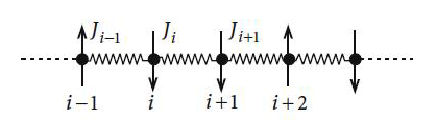
\includegraphics[scale=0.5]{./ising-pics/ising01.png}
  \caption{1-D Ising-Modell-Kette (Quelle: W. Nolting - Grundkurs Theo-
retische Physik: Band 6)
}
  \label{fig:1}
\end{figure}


Die Hamiltonfunktion dieses Systems lautet

\begin{align}
  \label{eq:1}
  H = -\sum_{ij}J_{ij}S_iS_j - \vec \mu \vec B \sum_i S_i
\end{align}

Dabei ist \(J_{ij} \) eine Wechselwirkungskonstante die die magnetische Wechselwirkung zwischen den Teilchen \(i\) und \(j\) beschreibt. \(S_i=\pm 1\) ist dazu da um das Vorzeichen des Spins darzustellen. \(\vec mu\) ist dabei das Magnetische Moment und \(\vec B\) die magnetische Flussdichte. 

Wir betrachten das Magnetfeld in z-Richtung, d.h. \(\vec B = (0,0,B_0)^T\), weiterhin gilt im Ising-Modell nur die Wechselwirkung zwischen benachbarten Teilchen \(j=i+1\), vereinfacht sich die Gleichung (\ref{eq:1}) insgesamt zu

\begin{align}
  \label{eq:2}
  H = -\sum_{i}^{N-1}J_{i}S_iS_{i+1} - \mu B_0 \sum_i S_i
\end{align}

\subsection*{1-D Ising-Modell ohne äußeres Magnetfeld ($B_0=0$)}

In diesem Abschnitt wollen wir untersuchen ob es bei einer kritischen Temperatur \(T_C\) zu einem Phasenübergang kommt. D.h. ob sich eine spontane Magnetisiertung einstellt. Dies war der ursprüngliche Plan von Ernst Ising, als dieses Modell erarbeitet hat.

Wir bestimmen zunächst die kanonische Zustandssumme, die allgemein lautet

\begin{align}
  \label{eq:3}
  Z = \sum_{\{\alpha\}} e^{-\beta E_\alpha} \text{ mit }\beta = \frac{1}{k_B T}
\end{align}

Setzen wir nun den Hamiltonoperator aus Gleichung (\ref{eq:2}) mit \(B_0=0\) in die Zustandssumme (\ref{eq:3}) ein, so lautet die von Teilchenzahl abhängige Zustandssumme

\begin{align}
  \label{eq:4}
    Z_N &= \sum_{S_1=\pm 1}\cdot\sum_{S_2=\pm 1}\cdots\sum_{S_N=\pm 1}  e^{\beta \sum_{i}^{N-1}J_{i}S_iS_{i+1}} \notag\\
&= \sum_{S_1=\pm 1}\cdot\sum_{S_2=\pm 1} e^{\beta J_{1}S_{1}S_2}\sum_{S_3=\pm 1}e^{\beta J_{2} S_2 S_3} \cdots\sum_{S_N=\pm 1}  e^{\beta J_{N-1}S_{N-1}S_{N}} \notag\\
&= \sum_{S_1=\pm 1}\prod_{i=2}^N\left( \sum_{S_i=\pm 1} e^{\beta J_{i-1}S_{i-1}S_i}\right) \notag\\
&= \sum_{S_1=\pm 1}\prod_{i=2}^N\left( e^{ + \beta J_{i-1}S_{i-1}}+ e^{ - \beta J_{i-1}S_{i-1}} \right)\notag\\
&= \sum_{S_1=\pm 1}\prod_{i=2}^N2\cosh( \beta J_{i-1}S_{i-1})
\end{align}


Nun möchten wir die erste Summe \(\sum_{S_1=\pm 1}\) berechnen. Das ist die Summe für das erste Teilchen das ohne Partner, d.h. ohne Wechselwirkung mit der Wechselwirkungskonstenen \(J_0=0\) und aus dem Grund müsste Die Exponentialfunktion lauten \(e^0\) und die Summe \(\sum_{S_1}e^0 = 2\). Rein mathematisch können wir aus der Gleichung (\ref{eq:4}) ein Produkt ausklammern

\begin{align}
  \label{eq:6}
   Z_N &=\sum_{S_1=\pm 1}\left( 2\cosh(\beta J_1 S_1) \prod_{i=3}^N2\cosh( \beta J_{i-1}S_{i-1}) \right) \notag\\
&=2\cosh(\beta J_1 1)\prod_{i=3}^N2\cosh( \beta J_{i-1}S_{i-1}) + 2\cosh(\beta J_1 (-1))\prod_{i=3}^N2\cosh( \beta J_{i-1}S_{i-1})
\end{align}

Mit der Relation  \(\cosh(\pm x) = \cosh(x) \) können wir die zwei Terme wieder zusammenfassen

\begin{align}
  \label{eq:7}
   Z_N &=2\cdot  2\cosh(\beta J_1)\prod_{i=3}^N2\cosh( \beta J_{i-1}S_{i-1})  \notag\\
&=2\cdot\prod_{i=2}^N2\cosh( \beta J_{i-1}S_{i-1}) = 2\cdot\prod_{i=2}^N2\cosh(\pm \beta J_{i-1}) \notag\\
&=  2\cdot\prod_{i=2}^N2\cosh(\beta J_{i-1})
\end{align}

Um die Gleichung (\ref{eq:7}) weiter zu vereinfachen, betrachten wir eine isotrope Wechselwirkung zwischen den Spins, d.h es gilt \(J_1=J_2=\dots=J_j=J\) mit \(j=2...N\). Desweiteren gilt \(\cosh(\beta J S_i ) = \cosh(\pm \beta J) =  \cosh(\beta J) \). Mit diesen Vereinfachungen lautet die Gleichung (\ref{eq:7})

\begin{align}
  \label{eq:5}
   Z_N =2\cdot \prod_{i=2}^N2\cosh( \beta J ) = 2\cdot \prod_{i=1}^{N-1}2\cosh( \beta J ) = 2\cdot 2^{N-1}\cosh^{N-1}( \beta J ) 
\end{align}

Aus Gleichung (\ref{eq:5}) erhalten wir schlussendlich eine Zustandssumme für ein 1-Dim. Ising-Modell ohne äußeres Magnetfeld

\begin{align}
  \label{eq:8}
  \boxed{Z_N = 2^{N}\cosh^{N-1}( \beta J )  }
\end{align}

\subsubsection*{Magnetisierung}

Um die Magnetisierung bestimmen zu können, müssen wir den Erwartungswert, bzw. den Mittelwert von Spineinstellung \(\langle S_i\rangle =\langle S\rangle \) bestimmen, da er laut der Beziehung

\begin{align}
  \label{eq:9}
  M_S(T) = \mu \langle S\rangle
\end{align}

Direkt proportional zu der Magnetisierung ist. Es ist geschickt den Mittelwert bzw. den Erwartungswert der Spineinstellung \(S_i\) nicht direkt zu bestimmen sondern über die Spin-Spin-korrelation-Funktion

\begin{align}
  \label{eq:10}
  g_{i,i+j} = \langle S_iS_{i+j}\rangle - \langle S_i\rangle\langle S_{i+j}\rangle
\end{align}

Den es gilt für weit auseinander liegende Spins, dass diese unkorreliert sind, d.h \(j\to\infty\) geht \(g_{i,i+j}\to 0\)

\begin{align}
  \label{eq:11}
   \lim_{j\to\infty} g_{i,i+j} = \lim_{j\to\infty}\left( \langle S_iS_{i+j}\rangle - \langle S_i\rangle\langle S_{i+j}\rangle\right) = 0 \notag\\
\Leftrightarrow \langle S_iS_{i+j}\rangle = \langle S_i\rangle\langle S_{i+j}\rangle = \langle S \rangle^2
\end{align}

Für den Erwartungswert \(\langle S_iS_{i+j}\rangle\) gilt allgemein

\begin{align}
  \label{eq:12}
  \langle S_iS_{i+j}\rangle &= \frac{1}{Z_N} \sum_{\{\alpha\}} S_i S_{i+j}  e^{\beta \sum_i^{N-1}J_iS_i S_{i+j} } \notag\\
&= \frac{1}{Z_N} \sum_{\{\alpha\}} S_i \cdot 1\cdot S_{i+j}  e^{\beta \sum_i^{N-1}J_iS_i S_{i+j} } \notag\\
&= \frac{1}{Z_N} \sum_{\{\alpha\}} (S_i\underbr{S_{i+1})(S_{i+1}}_{=1}\underbr{S_{i+2})(S_{i+2}}_{=1}\underbr{S_{i+3})}_{=1}\cdots\underbr{(S_{i+j-1}}_{=1} S_{i+j})  e^{\beta \sum_i^{N-1}J_iS_i S_{i+j} } 
\end{align}

Den Erwartungwert können wir durch ableiten der Zustandsumme nach \(\beta J_i\) gewinnen. Um die Wechselwirkung zwischen Spin \(i\) und Spin \(j\) zu bekommen, muss man alle Ableitungen zwischen dem \(i\)-ten und dem \((i+j-1)\)-ten Spin auf die Zustandsumme anwenden.

\begin{align}
  \label{eq:13}
  \langle S_iS_{i+j}\rangle &=  \frac{1}{Z_N} \pdiff_{(\beta J_i)}\pdiff_{(\beta J_{i+1})}\cdots \pdiff_{(\beta J_{i+j-1})} Z_N \notag\\
&\stackrel{~(\ref{eq:7})}=  \frac{1}{Z_N} \pdiff_{(\beta J_i)}\pdiff_{(\beta J_{i+1})}\cdots \pdiff_{(\beta J_{i+j-1})} \left(2\cdot\prod_{i=2}^N2\cosh( \beta J_{i-1})\right)  \notag\\
&=\cancel{\frac{\cosh(\beta J_{1})\cdots \cosh(\beta J_{i-1})}{ \cosh(\beta J_{1})\cdots \cosh(\beta J_{i-1})} } \times\notag \\
&\qquad\times \frac{ \sinh(\beta J_{i})\cdots\sinh(\beta J_{i+j-1})}{\cosh(\beta J_{i})\cdots\cosh(\beta J_{i+j-1})}\notag \\
&\qquad \times \cancel{ \frac{  \cosh(\beta J_{i+j}) \cdots \cosh(\beta J_{N})  }{   \cosh(\beta J_{i+j}) \cdots \cosh(\beta J_{N}) }} \notag\\
%
&=\prod_{k=i}^{i+j-1} \tanh(\beta J_{k}) = \prod_{k=1}^{j} \tanh(\beta J_{k})
\end{align}

Wegen Isotroper Wechselwirkung können wir das Produkt aus Gleichung (\ref{eq:13}) als Potenz schreiben

\begin{align}
  \label{eq:14}
   \langle S_iS_{i+j}\rangle =  \tanh^j(\beta J)
\end{align}

Laut Gleichung (\ref{eq:10}) für \(j\to\infty\) gilt

\begin{align}
  \label{eq:15}
\langle S \rangle^2 =  \langle S_i\rangle\langle S_{i+j}\rangle = \lim_{j\to\infty} \tanh^j(\beta J)
\end{align}

Betrachten wir die Magnetisierung aus Gleichung (\ref{eq:9}), so können wir schreiben

\begin{align}
  \label{eq:16}
  M(T) = \mu \lim_{j\to\infty} \tanh^{j/2}(\beta J)
\end{align}

\begin{itemize}
\item Die Magnetisierung für \(T>0\) ist immer Null, da \(\lim_{y\to\infty}\tanh^y(x)=0\)
\item Die Magnetisierung für \(T=0\) ist gleich \(\mu\) da \(\lim_{y\to\infty}\tanh^y(\infty)=1^\infty=1\)
\end{itemize}

Somit stellt sich \textit{keine spontane Magnetisierung} für endliche Temperaturen ein.\\

Der Erwartungswert aus Gleichung (\ref{eq:15}) ist Null für \(\beta J=\frac{1}{k_BT} J \ne \infty \) , d.h. für jede Temperatur \(T\ne 0\). Daraus folgt dass der gemittelte Spinzustand \(\langle S \rangle\)  auch Null ist. Was zu erwarten ist, da bei endlichen Temperaturen die Spinzustände zufällig chaotisch zwischen \(+ 1\) und \(-1\) verteilt sind. Somit muss der statistische Mittelwert bei Null liegen.


\subsection*{1D-Ising-Modell mit Magnetfeld $B_0\ne 0$}

Nun wollen wir die Zustandssumme für das 1D-Ising-Modell berechnen. Dazu benutzen wir die sogenannte Transfer-Matrix-Methode. Als Randbedingung gilt auch weiterhin dass jedes Spin nur mit seinem Nachbarn wechselwirken kann und die Wechselwirkung ist jetzt von beginn an isotrop, das bedeutet \(J_i = J\). Hinzu kommt dass die Kette geschlossen wird, d.h. Das letzte Element ist nun benachbart mit dem ersten Element

\begin{align}
  \label{eq:17}
  S_{N+1} = S_1
\end{align}

Die Vollständige Hamiltonfunktion aus Gleichung (\ref{eq:2}) lautet

\begin{align}
  \label{eq:18}
    H = - J \sum_{i}^{N-1} S_iS_{i+1} - \mu B_0 \sum_i S_i
\end{align}

Die allgemeine Zustandssumme lautet

\begin{align}
  \label{eq:19}
  Z_N &= \sum_{\{S\}} e^{\beta J \sum_{i}^{N-1} S_iS_{i+1} + \beta \mu B_0 \sum_i S_i }  \notag\\
&=\sum_{S_1=\pm 1}\sum_{S_2=\pm 1}\cdots \sum_{S_N=\pm 1} e^{(\beta J S_1 S_{2} + \beta \mu B_0 S_1) + (\beta J S_2 S_{3} + \beta \mu B_0 S_2) +\dots+ (\beta J S_N S_{N+1} + \beta \mu B_0 S_N) } 
\end{align}

Wir formen die Zustandssumme noch etwas um, damit man ein physikalisches Verhalten bezüglich des Magnetfeldes  zwischen den Spins identifizieren kann (siehe Tabelle \ref{tab:1}).  Mit der Randbedinung aus Gleichung (\ref{eq:17}) ersetzen wir \(S_{N+1}\) durch \(S_1\) und erhalten

\begin{align}
  \label{eq:20}
   Z_N &=\sum_{S_1=\pm 1}\sum_{S_2=\pm 1}\cdots \sum_{S_N=\pm 1} e^{(\beta J S_1 S_{2} + \beta \mu B_0 S_1) + (\beta J S_2 S_{3} + \beta \mu B_0 S_2) +\dots+ (\beta J S_N S_1 + \beta \mu B_0 S_N) } \notag\\
&=\sum_{S_1=\pm 1}\sum_{S_2=\pm 1}\cdots \sum_{S_N=\pm 1} e^{(\beta J S_1 S_{2} + \beta \mu B_0\frac{1}{2}(S_1+S_1)) + (\beta J S_2 S_{3} + \beta \mu B_0 \frac{1}{2}(S_2+S_2)) +\dots+ (\beta J S_N S_1 + \beta \mu B_0 \frac{1}{2}(S_N+S_N)) } \notag\\
&=\sum_{S_1=\pm 1}\sum_{S_2=\pm 1}\cdots \sum_{S_N=\pm 1} e^{(\beta J S_1 S_{2} + \beta \mu B_0\frac{1}{2}(S_1+S_2)) + (\beta J S_2 S_{3} + \beta \mu B_0 \frac{1}{2}(S_2+S_3)) +\dots+ (\beta J S_N S_1 + \beta \mu B_0 \frac{1}{2}(S_N+S_1)) } \notag\\
&=\sum_{S_1=\pm 1}\sum_{S_2=\pm 1}\cdots \sum_{S_N=\pm 1} e^{(\beta J S_1 S_{2} + \beta \mu B_0\frac{1}{2}(S_1+S_2))}e^{(\beta J S_2 S_{3} + \beta \mu B_0 \frac{1}{2}(S_2+S_3))}\cdots e^{(\beta J S_N S_1 + \beta \mu B_0 \frac{1}{2}(S_N+S_1)) } \notag\\
\end{align}

Man sieht wenn die Spins antiparallel sind, z.B. \(S_1=+1\) und \(S_2=-1\) dann verschwindet das Magnetfeld im Exponenten. Wenn die Beide positiv sind, dann erhält man auch ein positives Magnetfeld und entsprechend erhält man ein negatives Magnetfeld wenn beide Spins negativ sind.  Nun definieren wir die sogenannte Transfer-Funktoin \(T_{i,i+1}\)

\begin{align}
  \label{eq:21}
  T_{i,i+1}= e^{(\beta J S_i S_{i+1} + \beta \mu B_0\frac{1}{2}(S_i+S_{i+1}))}
\end{align}

Damit lautet die Gleichung (\ref{eq:20})

\begin{align}
  \label{eq:22}
   Z_N &=\sum_{S_1=\pm 1}\sum_{S_2=\pm 1}\cdots \sum_{S_N=\pm 1} T_{1,2}\cdot T_{2,3}\cdots T_{N,1}
\end{align}

Die Transfer-Funktion \(T_{i,i+1}\) kann man als eine \(2\times 2\)-Matrix schreiben, da es 4 verschiedene Kombinationen bei 2 interaggierenden Spins an Spinzuständen gibt

\begin{table}[h]
  \centering
  \begin{tabular}{ccc}
    i&i+1&\( e^{(\beta J S_i S_{i+1} + \beta \mu B_0\frac{1}{2}(S_i+S_{i+1}))} \) \\
\hline
\hline
    \(\uparrow\)&\(\uparrow\)& \( e^{\beta J  + \beta \mu B_0 } \)  \\
\hline
    \(\uparrow\)&\(\downarrow\)& \( e^{-\beta J } \)   \\
\hline
    \(\downarrow\)&\(\uparrow\)& \( e^{-\beta J } \)  \\
\hline
    \(\downarrow\)&\(\downarrow\)& \( e^{\beta J  - \beta \mu B_0 } \)
  \end{tabular}
  \caption{Mögliche Spin-Kombinationen}
  \label{tab:1}
\end{table}

Damit lässt sich die Transfer-Matrix schreiben als

\begin{align}
  \label{eq:23}
\hat T =
\begin{pmatrix}
   \uparrow \uparrow&  \uparrow\downarrow \\
   \downarrow\uparrow& \downarrow\downarrow
\end{pmatrix} = 
\begin{pmatrix}
  e^{\beta J  + \beta \mu B_0 }&e^{-\beta J }\\
 e^{-\beta J }&e^{\beta J  - \beta \mu B_0 }
\end{pmatrix}
\end{align}

Mit den zugehörigen Spinzuständen

\begin{align}
  \label{eq:24}
  \ket{S_i} = \ket{\uparrow} \equiv
  \begin{pmatrix}
    1\\0
  \end{pmatrix}
\qquad
  \ket{S_i} = \ket{\downarrow} \equiv
  \begin{pmatrix}
    0\\1
  \end{pmatrix}
\end{align}

Mit Hilfe der Transfer-Matrix können wir die Transfer-Funktion schreiben

\begin{align}
  \label{eq:25}
  T_{i,i+1} =  \bra{S_i} \hat T \ket{S_{i+1}}
\end{align}

Setzen wir nun die Definition (\ref{eq:25}) in die Zustandsfunktion aus Gleichung (\ref{eq:22}) ein

\begin{align}
  \label{eq:26}
  Z_N &=\sum_{S_1=\pm 1}\sum_{S_2=\pm 1}\cdots \sum_{S_N=\pm 1} T_{1,2}\cdot T_{2,3}\cdots T_{N,1} \notag \\
&=\sum_{S_1=\pm 1}\sum_{S_2=\pm 1}\cdots \sum_{S_N=\pm 1}\bra{S_1} \hat T \underbr{\ket{S_{2}} \bra{S_2}}_{\mathds 1_2} \hat T \underbr{\ket{S_{3}} \hphantom{\bra{S_3}} }_{\mathds 1_2}\cdots\underbr{\hphantom{\bra{S_N} } \bra{S_N}}_{\mathds 1_2} \hat T \ket{S_{1}}
\end{align}

Aufgrund der Vollständigkeits-Relation \(\sum_{S_i}\ket{S_i}\bra{S_i}=\mathds 1_2 \) kann die Zustandssumme (\ref{eq:26}) weiter vereinfacht werden

\begin{align}
  \label{eq:27}
  Z_N &=\sum_{S_1=\pm 1} \bra{S_1} \hat T^N \ket{S_1} =  \bra{\uparrow} \hat T^N \ket{\uparrow} +  \bra{\downarrow} \hat T^N \ket{\downarrow} = \text{Tr}\left( \hat T^N \right)
\end{align}

Da die Spur unabhängig von der gewählten Basis ist, können wir die Matrix \(\hat T\) diagonalisieren um weitere Erkenntnisse zu gewinnen. Die Zustandssumme ist dann die Summe der Diagonalelemente bzw. der Eigenwerte der Matrix

\begin{align}
  \label{eq:28}
  Z_N &= \text{Tr}\left( \hat T^N \right) = 
\text{Tr}\left(
  \begin{pmatrix}
    \lambda_1&0\\
0&\lambda_2
  \end{pmatrix}^N
\right)=
\lambda_1^N +  \lambda_2^N
\end{align}

Die Eigenwerte \(\lambda_i\) der Matrix werden durch die Bedingung \(det|\hat T - \lambda\cdot\mathds 1_2|\stackrel{!}=0\) berechnet

\begin{align}
  \label{eq:29}
\left(  e^{\beta J  + \beta \mu B_0 } -\lambda  \right) \left( e^{\beta J  - \beta \mu B_0 } -\lambda  \right) - e^{-2\beta J}\stackrel{!}=0 \notag\\
\Leftrightarrow e^{2\beta J} - \lambda e^{\beta J  + \beta \mu B_0 } - \lambda e^{\beta J  - \beta \mu B_0 } + \lambda^2 - e^{-2\beta J} =0 \notag\\
\Leftrightarrow \lambda^2 - \lambda (\underbr{e^{\beta J  + \beta \mu B_0 } + \lambda e^{\beta J  - \beta \mu B_0 }}_{e^{\beta J}2\cosh(\beta \mu B_0 ) }) + \underbr{ e^{2\beta J} - e^{-2\beta J}}_{2\sinh(2\beta J)} =0 \notag\\
\Leftrightarrow \lambda^2 - \lambda 2 e^{\beta J}\cosh(\beta \mu B_0 )  + 2\sinh(2\beta J) =0 \notag\\
\end{align}

Mit Hilfe der Mitternachtsformel folgt

\begin{align}
  \label{eq:30}
  \lambda_{1,2} &= \frac{ e^{\beta J}2\cosh(\beta \mu B_0)\pm \sqrt{e^{2\beta J}4\cosh^2(\beta \mu B_0) - 4\cdot 2\sinh(2\beta J)  } }{2} \notag\\
&=  e^{\beta J}\cosh(\beta \mu B_0)\pm \sqrt{e^{2\beta J}\cosh^2(\beta \mu B_0) - e^{2\beta J} + e^{-2\beta J}   }  \notag\\
&=  e^{\beta J}\left[\cosh(\beta \mu B_0)\pm \sqrt{\underbr{\cosh^2(\beta \mu B_0) - 1}_{\sinh^2(\beta \mu B_0)} + e^{-4\beta J}   } \right] 
\end{align}

Somit erhalten wir zwei Eigenwerte

\begin{align}
  \label{eq:31}
 \lambda_{1,2}  =  e^{\beta J}\left[\cosh(\beta \mu B_0)\pm \sqrt{\sinh^2(\beta \mu B_0) + e^{-4\beta J}   } \right]
\end{align}

Betrachten wir zusätzlich den Limes der Zustandssumme für \(N\to\infty\), dann können wir sagen dass nur der erste Eigenwert \(\lambda_1\) der der größere Eigenwert ist, gegenüber dem kleineren \(\lambda_2\) dominiert. Denn es gilt

\begin{align}
  \label{eq:32}
 \boxed{ Z_N = \lambda_1^N + \lambda_2^N = \lambda_1^N\left( 1 + \frac{\lambda_2^N}{\lambda_1^N}  \right) \stackrel{N\to\infty} = \lambda_1^N = e^{\beta J N}\left[\cosh(\beta \mu B_0)+ \sqrt{\sinh^2(\beta \mu B_0) + e^{-4\beta J}   } \right]^N  }
\end{align}

Wir wollen überprüfen ob wir aus Gleichung (\ref{eq:32}) die gleiche Zustandssumme bekommen wie in Gleichung (\ref{eq:8}) wenn wir das Magnetfeld \(B_0=0\) setzen. 

\begin{align}
  \label{eq:33}
  Z_N(T,B_0=0) = e^{\beta J N}\left[1+ \sqrt{ e^{-4\beta J}   } \right]^N = e^{\beta J N}+ e^{-\beta J N} =2^N\cosh^N(\beta J)
\end{align}

Wie man sieht erhalten wir die selbe Zustandssumme im termodynamischen Limes \(N\to\infty\)  ohne Magnetfeld wie Gleichung (\ref{eq:8}).

\subsubsection*{Magnetisierung}

Der Erwartungswert der Magnetisierung lässt sich aus der Zustandsumme bestimmen. Es gilt

\begin{align}
  \label{eq:34}
  M(T,B_0,N) &= \frac{1}{Z_N}  \sum_{\{S\}} (\textcolor{blue}{\mu \sum_i^N S_i} )  e^{\beta J \sum_{i}^{N-1} S_iS_{i+1} + \beta B_0 \textcolor{blue}{\mu \sum_i^N S_i} } \notag \\
&=  \frac{1}{Z_N} \frac{\partial Z_N}{\partial (\beta B_0)} =  \frac{\partial}{\partial (\beta B_0)}\ln(Z_N) = \frac{\partial}{\partial (\beta B_0)}\ln(\lambda_1^N) = N \frac{\partial}{\partial (\beta B_0)}\ln(\lambda_1) \notag\\
&= N \frac{1}{\lambda_1} \frac{\partial \lambda_1}{\partial (\beta B_0)}
\end{align}

Mit \(\lambda_1\) aus Gleichung (\ref{eq:31}) folgt

\begin{align}
  \label{eq:35}
  M(T,B_0,N) &= N\frac{ \pdiff_{(\beta B_0)}\left( \cancel{e^{\beta J}}\left[\cosh(\beta \mu B_0) + \sqrt{\sinh^2(\beta \mu B_0) + e^{-4\beta J}   } \right] \right) } 
{\cancel{e^{\beta J}}\left[\cosh(\beta \mu B_0) + \sqrt{\sinh^2(\beta \mu B_0) + e^{-4\beta J}   } \right] } \notag\\
&= N \frac{ \mu \sinh(\beta \mu B_0) + \frac{2\mu\sinh(\beta \mu B_0)\cosh(\beta \mu B_0) }{2 \sqrt{\sinh^2(\beta \mu B_0) + e^{-4\beta J}   }}  } 
{\cosh(\beta \mu B_0) + \sqrt{\sinh^2(\beta \mu B_0) + e^{-4\beta J}   }  } \notag\\
&=\frac{ N \mu \sinh(\beta \mu B_0)}{ \cosh(\beta \mu B_0) + \sqrt{\sinh^2(\beta \mu B_0) + e^{-4\beta J}   }  } \left( 1  + \frac{\cosh(\beta \mu B_0) }{\sqrt{\sinh^2(\beta \mu B_0) + e^{-4\beta J}   }}  \right) \notag\\
&=\frac{ N \mu \sinh(\beta \mu B_0)}{ \cancel{\cosh(\beta \mu B_0) + \sqrt{\sinh^2(\beta \mu B_0) + e^{-4\beta J}   } } } \left( \frac{\cancel{\sqrt{\sinh^2(\beta \mu B_0) + e^{-4\beta J}   }+\cosh(\beta \mu B_0)} }{\sqrt{\sinh^2(\beta \mu B_0) + e^{-4\beta J}   }}   \right)
\end{align}

Somit erhalten wir die Magnetisierung diesmal mit Magnetfeld

\begin{align}
  \label{eq:37}
 \boxed{ M(T,B_0,N)  =\frac{ N \mu \sinh(\beta \mu B_0)}{\sqrt{\sinh^2(\beta \mu B_0) + e^{-4\beta J}   }} }
\end{align}

Alternativ lässt sich die Magnetisierung auch mit Hilfe der freien Energie \(F(T,B_0,N)\) bestimmen. Es gilt

\begin{align}
  \label{eq:41}
  M(T,B_0,N) = - \frac{\partial F(T,B_0,N)}{\partial B_0}\qquad \text{mit } F(T,B_0,N) = - k_B T \ln Z_N
\end{align}

In Abbildung \ref{fig:2} haben wir die Magnetisierung aus Gleichung (\ref{eq:37}) in Abhängigkeit von \(B_0\) für zwei verschiedene Termperaturen aufgetragen. Man sieht dass beide Kurven durch den Ursprung gehen, d.h. für \(B_0=0\) gibt es keine spontane Magnetisierung, außer für \(T=0\). 

Für \(B_0\ne 0\) richten sich die einzelnen Spins in Richtung des Magnetfeldes, das bedeutet es handelt sich hier um Paramagnetismus. Desweiteren sieht man, dass sich für große \(B_0\) die Magnetisierung asymptotisch einem festen Wert \(N\mu\)  nähert. Das sieht man aus der Limesbetrachtung der Gleichung (\ref{eq:37})

\begin{align}
  \label{eq:36}
  M(T,B_0,N) = \lim_{B_0\to\infty} \frac{ N \mu \sinh(\beta \mu B_0)}{\sqrt{\sinh^2(\beta \mu B_0) + e^{-4\beta J}   }} = \frac{ N \mu \sinh(\beta \mu B_0)}{\sinh(\beta \mu B_0)} = N\mu
\end{align}

\begin{figure}
  \centering
  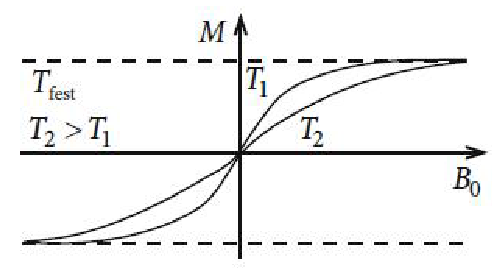
\includegraphics[scale=0.5]{./ising-pics/ising02.png}
  \caption{Magnetisierung in Abhängigkeit der Magnetfelddichte $B_0$ für verschiedene Temperaturen (Quelle: W. Nolting - Grundkurs Theo-
retische Physik: Band 6)
}
  \label{fig:2}
\end{figure}

\subsubsection*{Suszeptibilität $\chi_T(B_0)$}

Mit Hilfe der Magnetisierung in Gleichung (\ref{eq:37}) können wir die Suszeptibilität bestimmen. Die Suszeptibilität ist ein Maß für die Magnetisierbarkeit von Materialien in einem externen Magnetfeld. Sie ist folgendermaßen definiert

\begin{align}
  \label{eq:38}
  \chi_T = \left. \frac{\partial M(T,B_0,N)}{\partial H}\right|_{H=0} = \left. \frac{\mu_0 \partial M(T,B_0,N)}{\partial B_0}\right|_{B_0=0}
\end{align}

Mit der Gleichung (\ref{eq:37}) folgt

\begin{align}
  \label{eq:39}
  \chi_T &= \left. \mu_0 \pdiff_{B_0}  \frac{ N \mu \sinh(\beta \mu B_0)}{\sqrt{\sinh^2(\beta \mu B_0) + e^{-4\beta J}   }}  \right|_{B_0=0} \notag\\
&= \left. \mu_0 \frac{ N \mu^2 \beta \cosh(\beta \mu B_0)}{\sqrt{\sinh^2(\beta \mu B_0) + e^{-4\beta J}   }}  \right|_{B_0=0} -  \left. \mu_0 \frac{ N \mu \overbr{\sinh(\beta \mu^2 B_0)}^{=0 \text{ für }B_0=0}2\sinh(\beta \mu B_0)\cosh(\beta \mu B_0)\beta }{2(\sinh^2(\beta \mu B_0) + e^{-4\beta J}   )^{3/2}}  \right|_{B_0=0}  \notag\\
&=  \mu_0 \frac{ N \mu^2 \beta }{e^{-2\beta J}  } 
\end{align}

Somit erhalten wir für die Suszeptibilität

\begin{align}
  \label{eq:40}
 \boxed{ \chi_T = \frac{ \mu_0 \mu^2 N }{k_B T}e^{ \frac{2J}{k_B T}} }
\end{align}

Aus der Gleichung (\ref{eq:40}) sieht man, dass für \(T\to 0\) der Term \(\frac{1}{T}\) gegen \(\infty\) geht, heißt dass die Suszeptibilität den höchst möglichen Wert erreicht, was auf einen Phasenübergang bei \(T=0\) hindeutet. Aus der Abbildung \ref{fig:3} ersieht man, dass die inverse Suszeptibilität für höhere Temperaturen sich einer Geradengleichung annähert. Dies besagt auch das allseits beliebte Curie-Gesetzt \(\chi=\frac{C}{T}\) bzw. \(\frac{1}{\chi}=\frac{1}{C}T\) mit \(C\) der Curie-Konstante.

\begin{figure}
  \centering
  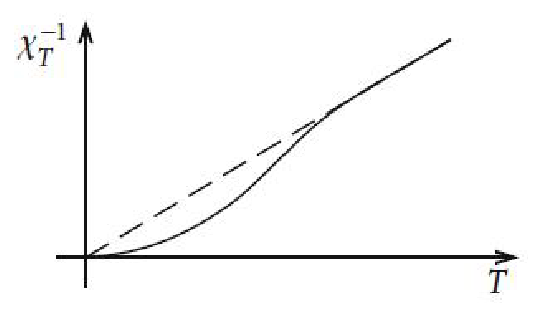
\includegraphics[scale=0.5]{./ising-pics/ising03.png}
  \caption{Kehrwert der Suszeptibilität in Abhängigkeit der Termperatur für \(B_0=0\)  (Quelle: W. Nolting - Grundkurs Theo-
retische Physik: Band 6)
}
  \label{fig:3}
\end{figure}




\end{document}
